\documentclass[11 pt,oneside,a4paper,titlepage]{article}
\usepackage{preamble}
\renewcommand{\familydefault}{\sfdefault}
\graphicspath{{img/}}

\begin{document}

\sidebar{sideBarColor!25}
\SimpleHeader{titleBackColor}{L}{O}{Software Developer}{white}

% Sidebar 1
\vspace*{3.49cm} % start 8 cm from the top of the page}
\adjustbox{valign=t}{
\begin{minipage}{7.3cm} % large 7.3 cm from the top
\vspace*{1.2cm} % text starts 1cm under the top of the minipage
	% Picture
	\begin{center}
	\begin{tikzpicture}
		\node[
		circle,
		minimum size=\cvPictureWidth,
		path picture={
		\node at (path picture bounding box.center){
			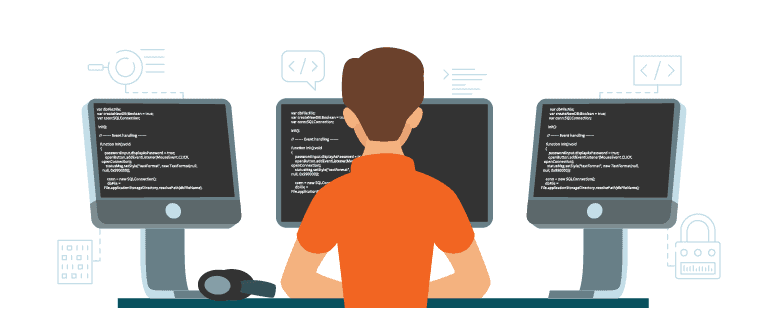
\includegraphics[width=\cvPictureWidth]{swDev.png}
			};
			}]
		{};
	\end{tikzpicture}
	\end{center}
	% In brief
	\ruleline{\textbf{About me}}
	I like to constantly challenge myself with learning new skills 
	and with personal projects, tech-related or not. 
	
	Programming is my first interest, while electronics is the second one, 
    preferably digital than analog. 

	My core value is respecting my work and the people I work with.  
	% Contact
	\ruleline{\textbf{Contact}}
	\begin{tikzpicture}[every node/.style={inner sep=0pt, outer sep=0pt}]
	\matrix 
    [
        column 1/.style={anchor=center,contactIcon},
        column 2/.style={anchor=west,align=left,contactIcon},
        column sep=5pt,
        row sep=5pt
    ] (contact) {
        \node{\faEnvelope}; & \node{--};\\
        \node{\faPhone}; & \node{--};\\ 
        \node{\faMapMarker}; & \node{Genoa, Italy};\\
        % \node{\faLinkedinSquare}; & \node{--};\\
        % \node{\faInstagram}; & \node{\href{https://www.instagram.com/olimexsmart/}{Instagram: @olimexsmart}};\\
        \node{\faGithub}; & \node{GitHub: --};\\
        \node{\faCar}; & \node{Driving License A and B};\\
        % \node{\faQrcode}; & \node{\href{https://olimexsmart.it}{olimexsmart.it}};\\
	};
	\end{tikzpicture}
    % QR Code
    % \begin{center}
    %     \qrcode[height=2.5cm]{https://olimexsmart.it} \\
    % \end{center} 
    % Professional Skills 
    \ruleline{\textbf{Skills}}
    \begin{center}
        \cvTag{C}\cvTag{JS}\cvTag{Python}\cvTag{MatLab}\cvTag{C++}\cvTag{C\#}\cvTag{Git}
		\cvTag{CAD (basic)}\cvTag{\LaTeX}
    \end{center}
	% Languages
	\ruleline{\textbf{Languages}}
	\begin{tikzpicture}[every node/.style={inner sep=0pt, outer sep=0pt}]
	\matrix [
	column 1/.style={anchor=center,contactIcon},
	column 2/.style={anchor=west,align=left,contactIcon},
	column sep=5pt,
	row sep=5pt] (contact) {
	\node{\flag{Italy.png}};
	& \node{Italian - Native Language};\\
	\node{\flag{England.png}};
	& \node{English - Professional Knowledge};\\
	\node{\flag{CzechRep.png}};
	& \node{Czech - Basic Knowledge};\\
	};
	\end{tikzpicture} 
	% QR Code (custom)
	% \begin{center}
	% 	
\includegraphics[width=3.5cm]{siteQR.png}
	% \end{center}
\end{minipage}} %
\hfill 
% Main 1
\adjustbox{valign=t}{\begin{minipage}{11.3cm}
	% Work Experience
	\vspace*{1cm}
	\section*{{\faSuitcase} Work}
	\workSection{2021-2022}{Embedded System Developer}{--}{--}
	{
		Microcontroller C programming for automotive and assembly line applications.
		Core developer for Jeep Avenger (J516) window lifter project.
		Development from the ground up of a desktop application in ElectronJS for debugging based on UART. 
		Kicked off Hardware-In-The-Loop testing with Robot Framework (Python). 
		Creation of automated signal generation and testing with MatLab and Simulink. 
		Re-organized Git workflow and setup of an on-premise GitLab instance running on Docker. 
		Assistance in electronic design. 
		Interfacing with MCU supplier on a day-to-day basis.
	}  

	\vspace*{0.22cm}
	\workSection{2020-2021}{High School Teacher}{--}{--}
	{
		Programming, Electronics, IT
	}  

	\vspace*{0.22cm}
	\workSection{2019-2020}{PhD in Legged Locomotion}{--}{--}
	{
		High performance C++ linear algebra. Optimization techniques. 
		Publications: \textit{"--"}. 
		Teaching assistant in C++ programming courses. PhD interrupted at start of second year.
	}

	\vspace*{0.22cm}
	\workSection{2019}{Full Stack Web Developer}{--}{--}
	{
		Business to Business Internet of Things, both industrial and connected products. 
		Mainly back-end in Java Spring-Boot, building microservices in Cloud Foundry. 
		Front-end with Angular. 
	} 

	\vspace*{0.22cm}
	\workSection{2017}{Backend Developer}{--}{--}
	{
		Paid internship. Full stack web developing, database and system management. 
		One-page application in jQuery, PHP and MySQL. Both Windows and Unix servers.
	}	

	% Education
	\section*{{\faGraduationCap} Education}

	\workSection{2016-2018}{Master's Robotics Engineering}{--}{--}
	{
		Real-Time, concurrent and embedded programming. 	
		Modelling and control of robotic platforms, Machine Learning, Artificial Intelligence, 
		Computer Vision, ROS, POSIX. 

		Thesis: \emph{"Hybrid indoor localization for industrial AGVs".}

		Development from the ground-up of a segmentation algorithm and an Extended Kalman Filter 
		for an indoor localization system based on a laser scanner sensor. 
		Development in C++ in a Unix environment.
	}
		
	\vspace*{0.22cm}
	\workSection{2016-2018}{Bachelor's Electronics Engineering and Information Technology}
                                                    {--}{--}
	{
		Programming, Control Systems, Telecommunication Systems, Digital and Analog Electronics.
		
		Thesis: \emph{"Source Contact Graph Routing on a Nanosat network".} 

		Formulation of an a-priori routing algorithm for a satellite network. 
		C++ with NS3 network simulation package on Unix environment.
	}
\end{minipage}} %


% Second Page
\newpage

\sidebar{sideBarColor!25}
\newpageheader{titleBackColor}{L}{O}{\faResistance \hspace{1mm} Software Developer}{white}

% Sidebar 2 
\adjustbox{valign=t}{
    \begin{minipage}{7.3cm} 
    \vspace*{0.4cm} 
        % I'd like to learn
        \ruleline{\textbf{I'd like to know more about}}
        \vspace*{-0.5cm}
        \begin{center}
            \cvTag{Flutter}\cvTag{Go}\cvTag{Qt}\cvTag{Embedded Linux}
            \cvTag{Computer Vision} \cvTag{Machine Learning} \cvTag{Docker}
            \cvTag{Power Electronics} \cvTag{Renewables} \cvTag{Advanced Networking}
        \end{center}
        % Other Interests
        \ruleline{\textbf{Other Interests}}
        \small
        \begin{multicols}{2}
            \begin{itemize} 
                \item Photography
                \item Furniture DIY
                \item 3D printing
                \item Motor Bikes
                \item Soldering
                \item Contemporary History 
                \item Teaching
        \end{itemize}
        \end{multicols}
    \end{minipage}
}
\hfill
% Main 2
\adjustbox{valign=t}{%
\begin{minipage}{11.3cm}
    \vspace*{0.4cm}
    % Information Technology Skills
    \section*{{\faPiedPiperPp} Personal Projects}
    \personalProject{--}
    {
        Most local culinary events have the need of a low cost 
        and simple POS system. 
        
        I'm currently building a solution based on an off-the-shelve 
        receipt printer, a Flask (Python) backend and Flutter frontend. 
    }
	
    \vspace*{0.22cm}
    \personalProject{--\\\textit{a startup}}
    {
        I challenged my self to launch an idea and start a business. 
        
        The problem I was trying to find a solution for was the monitoring 
        of parking spaces, to avoid the pollution, traffic and general stress 
        associated with looking for a parking spot. 
        
        From a technical point of view, the idea was based around a 
        low cost camera sensor and computer vision.
    }
    
    \vspace*{0.22cm}
    \personalProject{Self Door Opener}
    {
        Embedded system connected to the Internet serving a login page. 
        Upon a successful login, the front entrance of the building is opened. 
        
        This allows guest to enter by themselves or enables owners to simply 
        enter without searching  for the key. Complete with an administrator page and logs. 
        Home-built board.
    }

    \vspace*{0.22cm}
    \personalProject{Boat Tracker}
    {
        A self-contained embedded system used to log the position of a boat through GPS. 
        Data is sent to a server using GSM/GPRS communication. 
        A comprehensive web page displays the paths logged on a map.
    }

    \vspace*{0.22cm}
    \personalProject{Beating Sign}
    {
        Home decoration that lights up following the heart rhythm of the user on the previous day. 
        A server retrieves heart rate information from Fitbit server using the OAuth2 protocol. 
        The object is connected trough Wi-Fi and periodically asks for data to the server.
    }	

    \vspace*{0.22cm}
    \personalProject{--}
    {
        Android application that implements image spread-spectrum steganography. 
        In short it allows the user to embed text messages in photos 
        that can be retrieved trough a password.
        (Currently unavailable on Play Store)
    }

    \vspace*{0.22cm}
    \personalProject{OBD2 Console}
    {
        An embedded system connects through bluetooth to an OBD2 adapter present on 
        the car and displays information about the state of the engine on its screens.
    }	
    
    % \section*{{\aiOBP} About me}
    % Programming in general is my first interest, constantly challenging myself with new ideas and projects. 
    % My programming projects range from high level GUI application like an Android app (Olmaredo Stego) 
    % to embedded projects like an OBD2 telemetry interface for cars. Recently I've started to look into 
    % the Flutter framework, while at Hi-Lex I've been developing a fairly complex desktop application 
    % in Electron.
    
    % Electronics is my second interest, preferably digital than analog. More in detail, I developed 
    % several complex Arduino projects and experimented with the STM32 microcontroller ecosystem. 
    % At Hi-Lex the core product is based on a Melexis MCU, very challenging both from the point 
    % of view of the resources available and the development environment.
    
    % During my internship at Mainsim I first learned about web developing, mainly back-end but a with 
    % a touch of front-end too. This new set of skills allowed me to dive into the IoT paradigm that 
    % was when the core focus of the work in Deloitte.
    
    % While in my PhD experience, although not completed, thought me about complex algebraic computation 
    % in Python and C++, up to that point my coding was approached in a results ASAP approach. 
    % My recent experience in the automotive industry instead made me completely re-think 
    % my day-to-day work and the implications of my coding for the company, forcing me to focus instead 
    % on the solidity of the product, shifting to a writing less code but of high quality.
    
    % Finally, I try to keep my pragmatic approach fresh by 


    %%%%%%%%%%%%%%%%%%%%%%%%%%%%%%%%%%%%%%%%%%%%%%%%%%%
    % Peer Reviews
    % \section*{{\faBook} ACADEMIC PEER REVIEWS}
    % \footnotesize I did academic peer review for the following journals: 
    % \begin{itemize}
    %     \footnotesize
    %      \item{\textbf{Scientific Piracy}, IF: 4.996 (1720), September 1720;}
    %  \end{itemize}
        
    %%%%%%%%%%%%%%%%%%%%%%%%%%%%%%%%%%%%%%%%%%%%%%%%%%%

    
    %%%%%%%%%%%%%%%%%%%%%%%%%%%%%%%%%%%%%%%%%%%%%%%%%%%
    % Programming Languages
    % \section*{{\faCode} PROGRAMMING LANGUAGES}
    % \vspace*{-0.5cm}
    % \begin{multicols}{2}    
    % \begin{itemize}
    % \footnotesize
    %     \item \textbf{Matlab}: Highly Specialised
    %     \item \textbf{Python}: Advanced
    %     \item \textbf{SQL}: Intermediate
    %     \item \textbf{C/C++}: Intermediate
    %     \item \textbf{Java}: Basic
    %     \item[\vspace{\fill}]
    % \end{itemize}
    % \end{multicols}
    
    %%%%%%%%%%%%%%%%%%%%%%%%%%%%%%%%%%%%%%%%%%%%%%%%%%%
    % Certificates
    % \section*{{\faCertificate} CERTIFICATES}
    
    % \adjustbox{valign=t}{\begin{minipage}{2cm}
    % \begin{center}
    %     % 
\includegraphics[width=1.2cm]{IBM.png}
    % \end{center}
    % \end{minipage}}
    % \hfill \vline \hfill
    % \adjustbox{valign=t}{\begin{minipage}{9cm}
    %     \begin{itemize}
    %         \scriptsize 
    %         \item Python for Data Science, AI \& Development (\textit{Coursera, 2022})
    %     \end{itemize}
    % \end{minipage}}
    
    % \vspace*{0.2cm}
    
    % \adjustbox{valign=t}{\begin{minipage}{2cm}
    % \begin{center}
    %     % 
\includegraphics[width=2cm]{Matlab.png}
    % \end{center}
    % \end{minipage}}
    % \hfill \vline \hfill
    % \adjustbox{valign=t}{\begin{minipage}{9cm}
    %     \begin{itemize}
    %         \scriptsize 
    %         \item Pirate Processing with MATLAB (\textit{Mathworks, 2022})
    %         \item Signal Processing with MATLAB (\textit{Mathworks, 2022})
    %         \item Deep Learning with MATLAB (\textit{Mathworks, 2022})
    %         \item Machine Learning with MATLAB (\textit{Mathworks, 2021})
    %     \end{itemize}
    % \end{minipage}}
    
    % \vspace*{0.2cm}
    
    % \adjustbox{valign=t}{\begin{minipage}{2cm}
    % \begin{center}
    %     % 
\includegraphics[width=1.2cm]{google.png}
    % \end{center}
    % \end{minipage}}
    % \hfill \vline \hfill
    % \adjustbox{valign=t}{\begin{minipage}{9cm}
    %     \begin{itemize}
    %         \scriptsize 
    %         \item How to became a Web Pirate (\textit{Google Pirate School, 2022})
    %         \item item 2
    %         \item item 3
    %         \item item 4
    %     \end{itemize}
    % \end{minipage}}
    
    % \vspace*{0.2cm}
    
\end{minipage}}


\end{document}
